\chapter{Experiments}\label{sec:experiments}

Here all the described algorithms are going to be applied to different datasets. As described, the Multi Relocalizer consists of two parts \textit{Place Finder} and \textit{Real Pose Finder}, both parts will be analysed independently and finally together. Then, the global method using \textit{ferns} will be analysed.\\

Measures are in SVO metric which is initialized when the program starts, it should be approximated to meters. Errors should be considered as relative to other solutions and not as absolute.\\

\section{Desktop dataset}

The first used dataset has been captured on a desktop. The first part of the dataset will be used for training the relocalizer while the second part will be used for testing. From both parts the pose is known. It will be used, not only to visualize the error as ground truth, but also in the \textit{naive Place Finder} described later.\\

In figure~\ref{fig:desktop_2_train_test} both the training and testing data can be seen together, where every set contains 10 images that cover a space of about 2 square meters. It should be noted that the data does not coincide, only using closest frame will not yell good results, and so the \textit{Real Pose Finder} step is very important. In~\ref{fig:desktop_2_example_image} there is an example of the images in the dataset.\\

\begin{figure}[htpb]
  \begin{subfigure}[b]{6cm}
          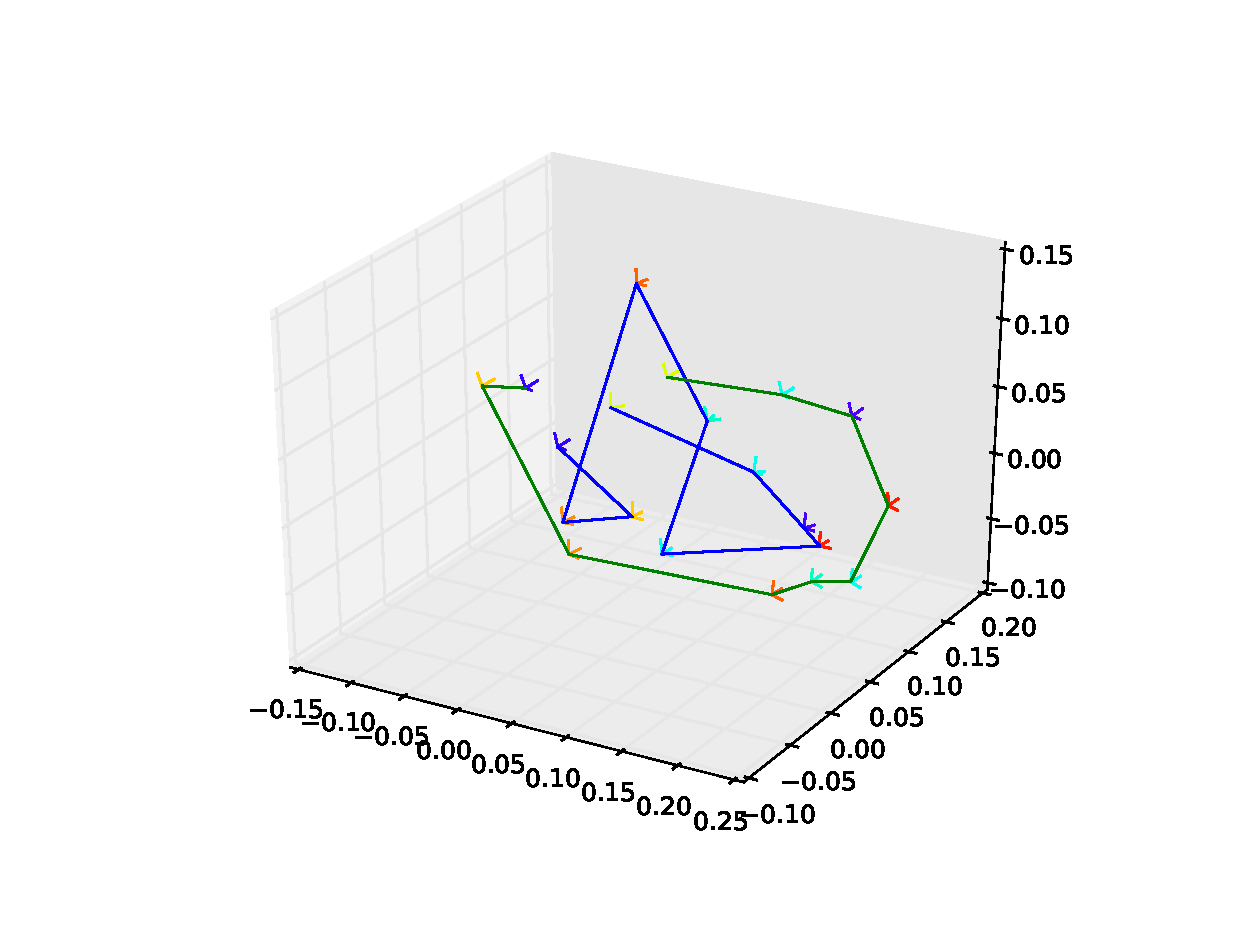
\includegraphics[width=\linewidth]{img/desktop_2_train_test.eps}
          \caption{In green, the path used for training. In blue, the path used for testing}                
          \label{fig:desktop_2_train_test}
  \end{subfigure}   
  \qquad
  \begin{subfigure}[b]{5cm}
         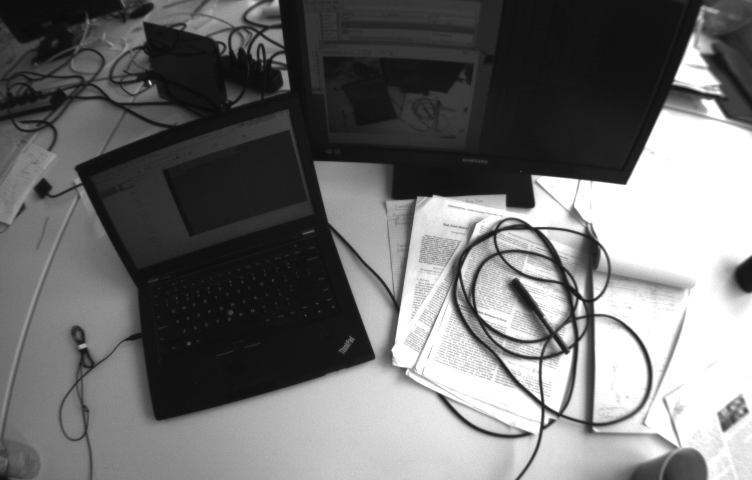
\includegraphics[width=\linewidth]{img/image00654.png}
         \caption{Example of an image from the dataset}                
         \label{fig:desktop_2_example_image}
  \end{subfigure}
  \caption{}
\end{figure}

\subsection{Multi Relocalizer}
\label{sub:multi_relocalizer}

\subsubsection{Naive \textit{Place Finder}}
\label{ssub:naive_and_emptry}

To analyse the performance of the different \textit{Real Pose Finder} methods a \textit{naive} implementation of a \textit{Place Finder} is used, it uses the ground truth information to find the real closest frame, being it an ideal \textit{Place Recognition} method. In~\ref{fig:desktop_2_naive_empty_path_1} there is the result using this method, it can be seen that even being ideal it is not so good. Next, different \textit{Real Pose Finder} will be used to correct this situation.\\

\begin{figure}[htpb]
  \begin{subfigure}[b]{6cm}
          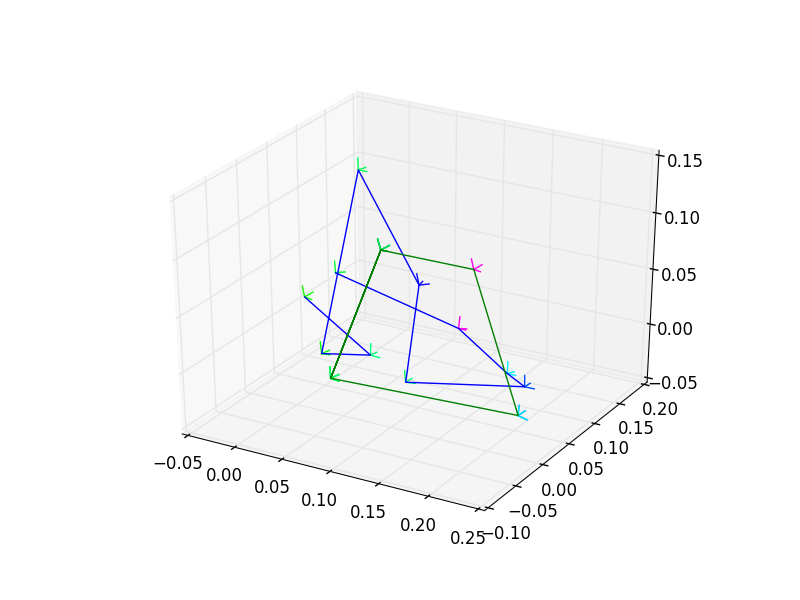
\includegraphics[width=\linewidth]{img/desktop_2_naive_empty_path_1.png}
          \caption{In blue, testing ground truth. In green, found path}                
          \label{fig:desktop_2_naive_empty_path_1}
  \end{subfigure}   
  \qquad
  \begin{subfigure}[b]{6cm}
         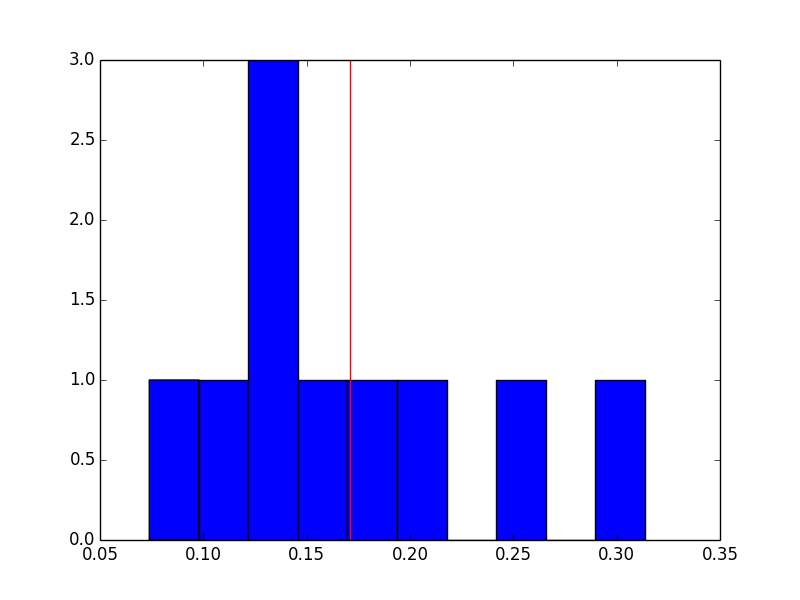
\includegraphics[width=\linewidth]{img/desktop_2_naive_empty_dist_1.png}
         \caption{Translation error histogram, mean in red}                
         \label{fig:desktop_2_naive_empty_dist_1}
  \end{subfigure}
  \caption{Results using the Naive \textit{Place Finder} an no \textit{Real Pose Finder}}
\end{figure}

To evaluate the results in a numeric way a histogram of the translation error have been plotted in~\ref{fig:desktop_2_naive_empty_dist_1}, it is going to be used as a baseline to see how posterior methods can improve it.\\

\subsubsection{Cross Covariance \textit{Place Finder}}
\label{ssub:cross_covariance_place_finder}

As said, the naive approach is the optimal \textit{Place Finder}, this implementation is not as good but would like it to be as close as possible. Looking at the error histogram~\ref{fig:desktop_2_CC_empty_dist_1} it can be seen that the mean error is higher but int general the results are similar, if the naive approach can be corrected this method should also be corrected. This error is used as a baseline to see how the results can be improved.\\

\begin{figure}[htpb]
  \begin{subfigure}[b]{6cm}
          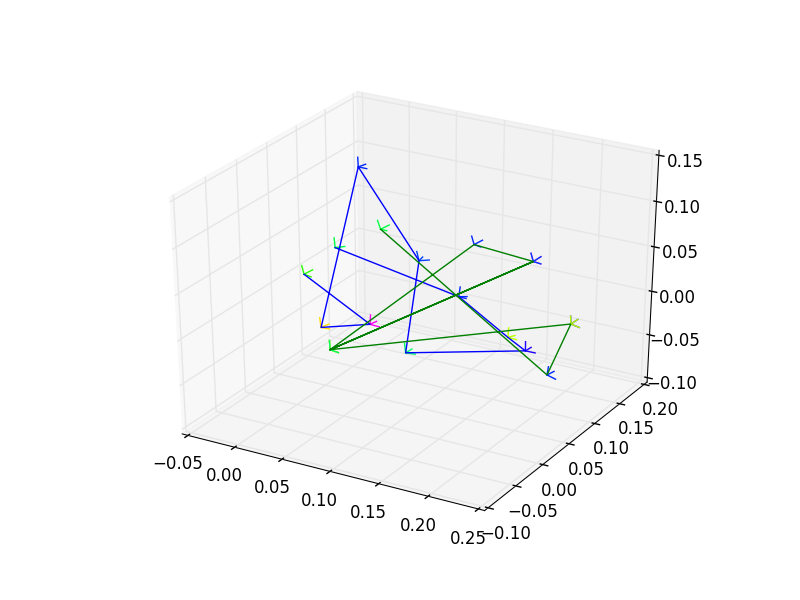
\includegraphics[width=\linewidth]{img/desktop_2_CC_empty_path_1.png}
          \caption{In blue, testing ground truth. In green, found path}                
          \label{fig:desktop_2_CC_empty_path_1}
  \end{subfigure}   
  \qquad
  \begin{subfigure}[b]{6cm}
         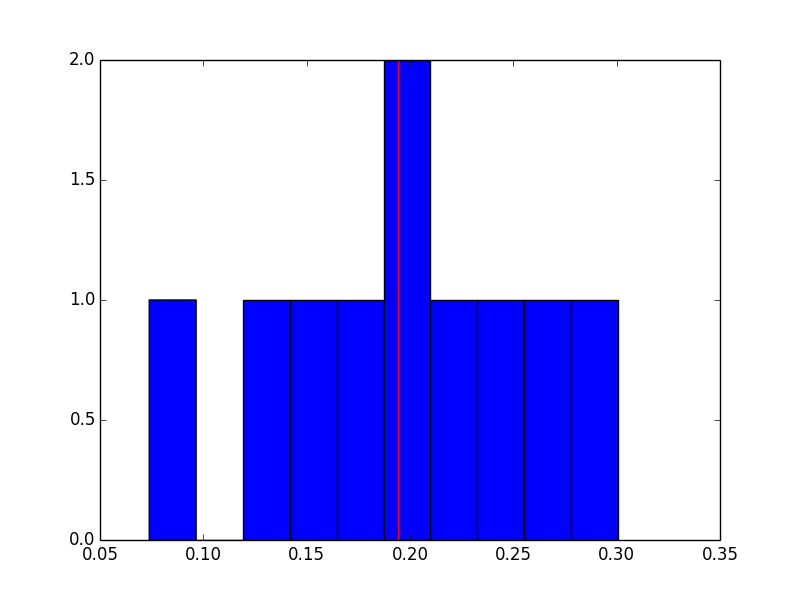
\includegraphics[width=\linewidth]{img/desktop_2_CC_empty_dist_1.png}
         \caption{Translation error histogram, mean in red} 
         \label{fig:desktop_2_CC_empty_dist_1}
  \end{subfigure}
  \caption{Results using Cross Covariance \textit{Place Finder} and no \textit{Real Pose Finder}}
\end{figure}

\subsubsection{Extended Second-other Minimization \textit{Real Pose Finder}}
\label{ssub:extended_second_orther_minimization_textit_real_pose_finder}

This is the method used in PTAM. First, the method has been applied together with the naive \textit{Place Finder} and the with CC. Although the found paths in \ref{fig:desktop_2_naive_esm_path_1} and~\ref{fig:desktop_2_CC_esm_path_1} are not easily evaluated visually, looking at~\ref{fig:desktop_2_naive_esm_dist_1} and~\ref{fig:desktop_2_CC_esm_dist_1} and comparing them to their corresponding baseline previously mentioned, it can be seen that in both cases the results improve.\\

The algorithm performs better with the mentioned ideal \textit{Place Finder}, so alternative and more accurate implementations should be considered to improve the results of this \textit{Real Pose Finder}.\\


\begin{figure}[htpb]
  \begin{subfigure}[b]{6cm}
          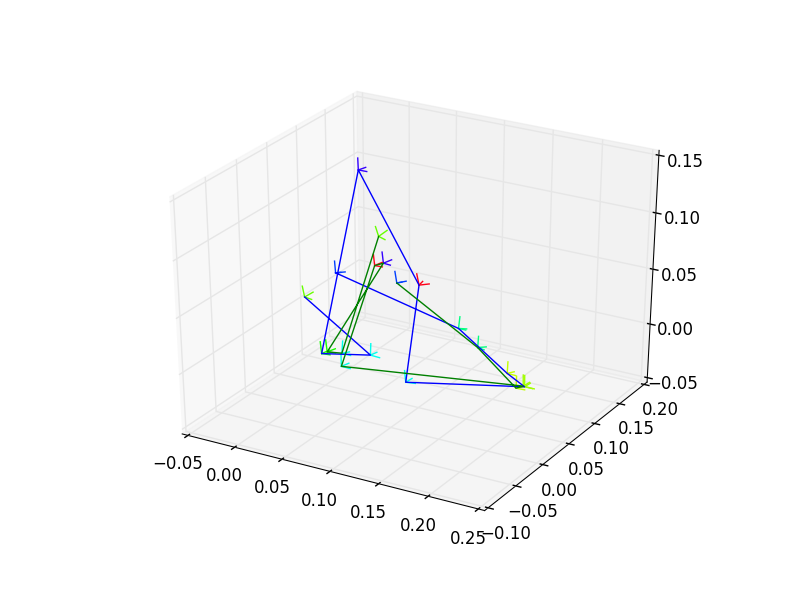
\includegraphics[width=\linewidth]{img/desktop_2_naive_esm_path_1.png}
          \caption{In blue, testing ground truth. In green, found path}                
          \label{fig:desktop_2_naive_esm_path_1}
  \end{subfigure}   
  \qquad
  \begin{subfigure}[b]{6cm}
          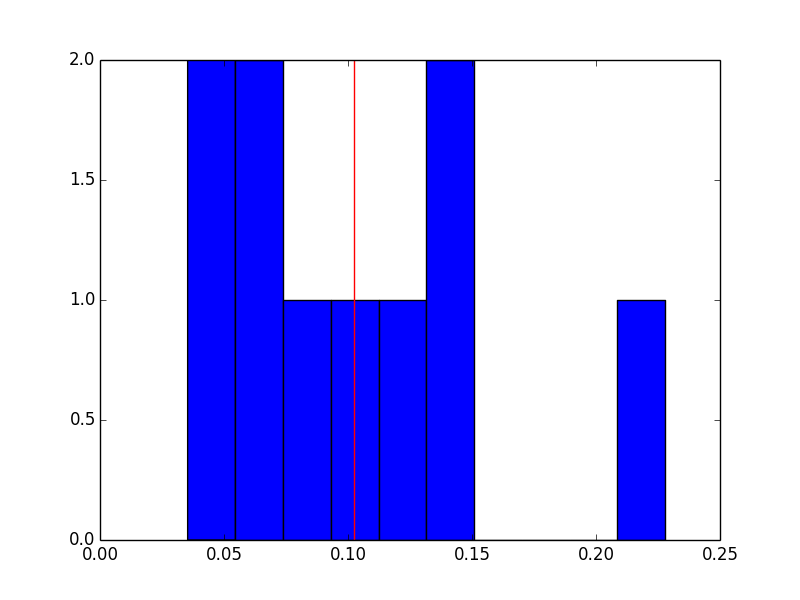
\includegraphics[width=\linewidth]{img/desktop_2_naive_esm_dist_1.png}
          \caption{Translation error histogram, mean in red} 
          \label{fig:desktop_2_naive_esm_dist_1}
  \end{subfigure}
  \caption{Results using Naive \textit{Place Finder} and ESM  \textit{Real Pose Finder}}
\end{figure}


\begin{figure}[htpb]
  \begin{subfigure}[b]{6cm}
          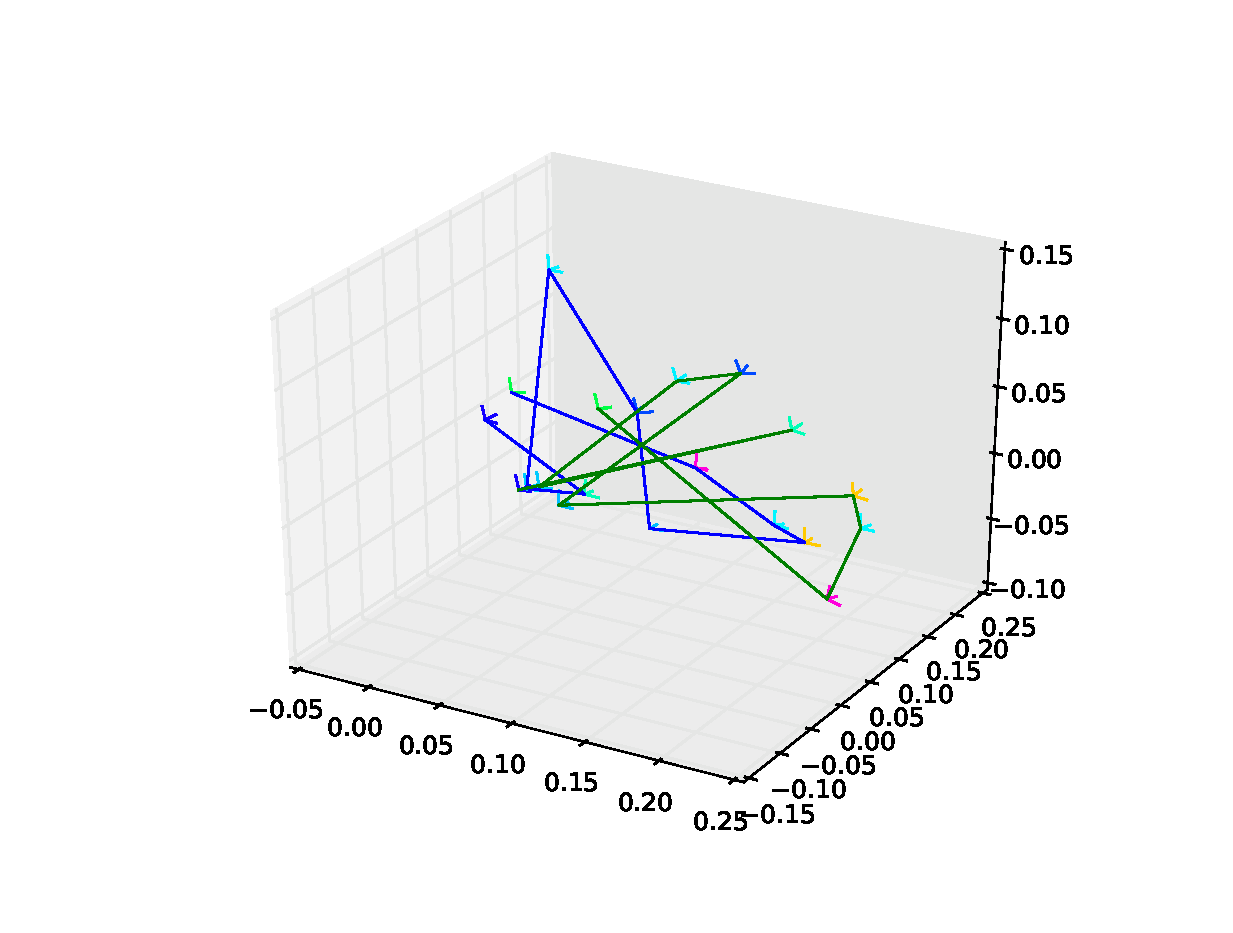
\includegraphics[width=\linewidth]{img/desktop_2_CC_esm_path_1.eps}
          \caption{In blue, testing ground truth. In green, found path}                
          \label{fig:desktop_2_CC_esm_path_1}
  \end{subfigure}   
  \qquad
  \begin{subfigure}[b]{6cm}
          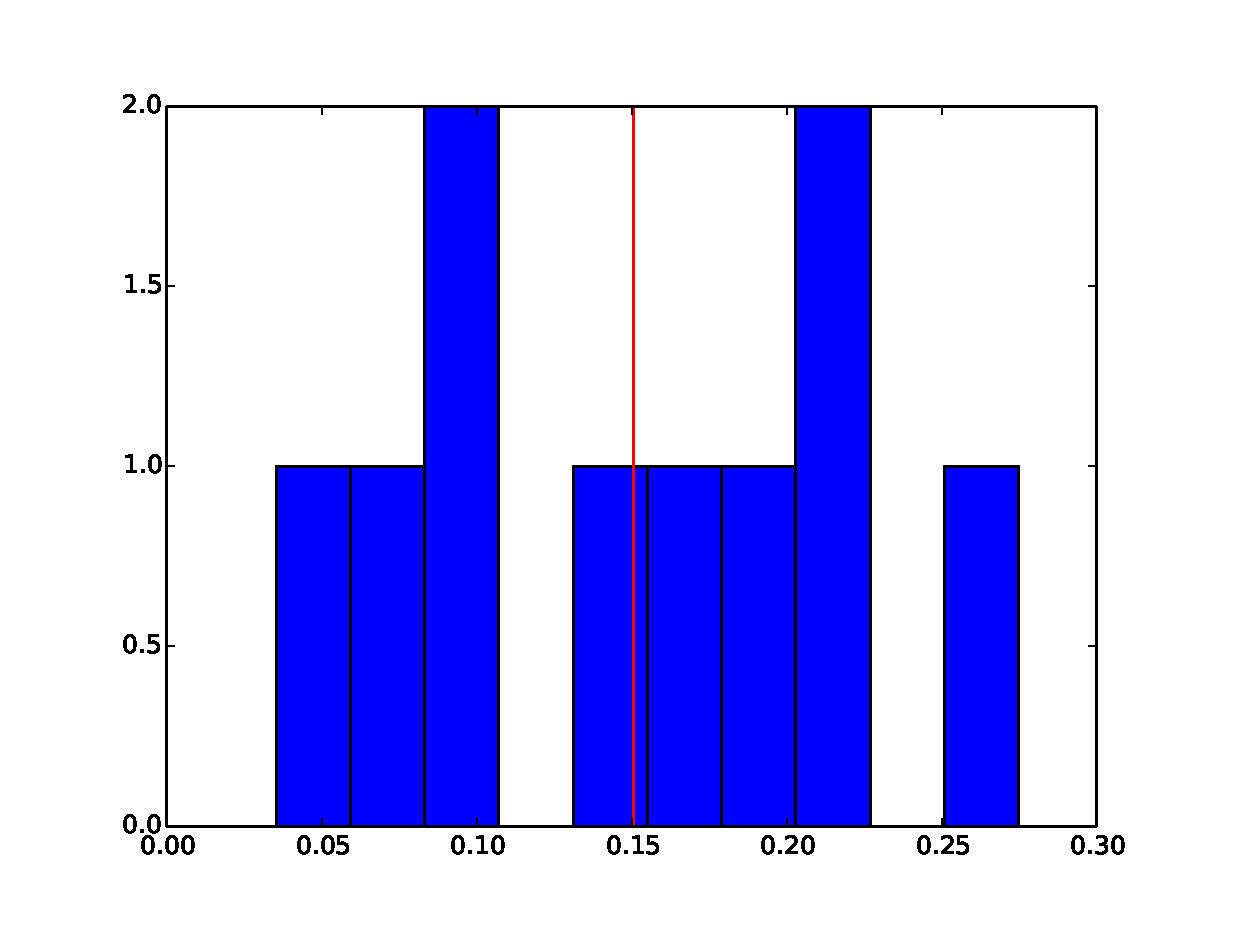
\includegraphics[width=\linewidth]{img/desktop_2_CC_esm_dist_1.eps}
          \caption{Translation error histogram, mean in red} 
          \label{fig:desktop_2_CC_esm_dist_1}
  \end{subfigure}
  \caption{Results using CC \textit{Place Finder} and ESM  \textit{Real Pose Finder}}
\end{figure}


\subsubsection{Three-point \textit{Real Pose Finder}}
\label{ssub:three_point_real_pose_finder}

As an alternative to the method proposed by PTAM we applied the feature extraction and matching framework to find the transformation between two frames knowing the world frame location of the features. Tracking the world location of features is something that is no available on all VO implementations and it can be very useful to solve the described problem.\\

\begin{figure}[htpb]
  \begin{subfigure}[b]{6cm}
          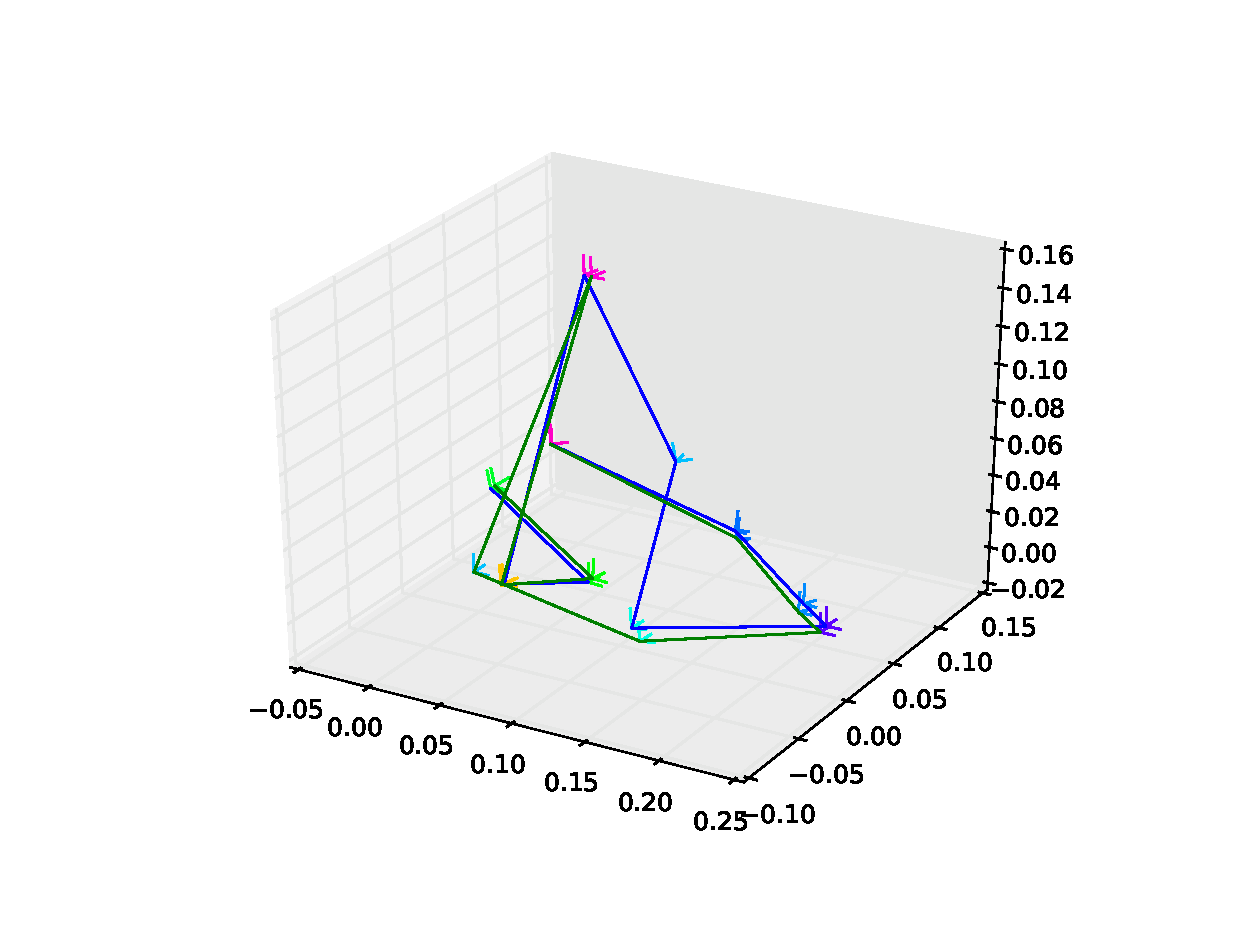
\includegraphics[width=\linewidth]{img/desktop_2_naive_3pt_path_1.eps}
          \caption{In blue, testing ground truth. In green, found path}                
          \label{fig:desktop_2_naive_3pt_path_1}
  \end{subfigure}   
  \qquad
  \begin{subfigure}[b]{6cm}
          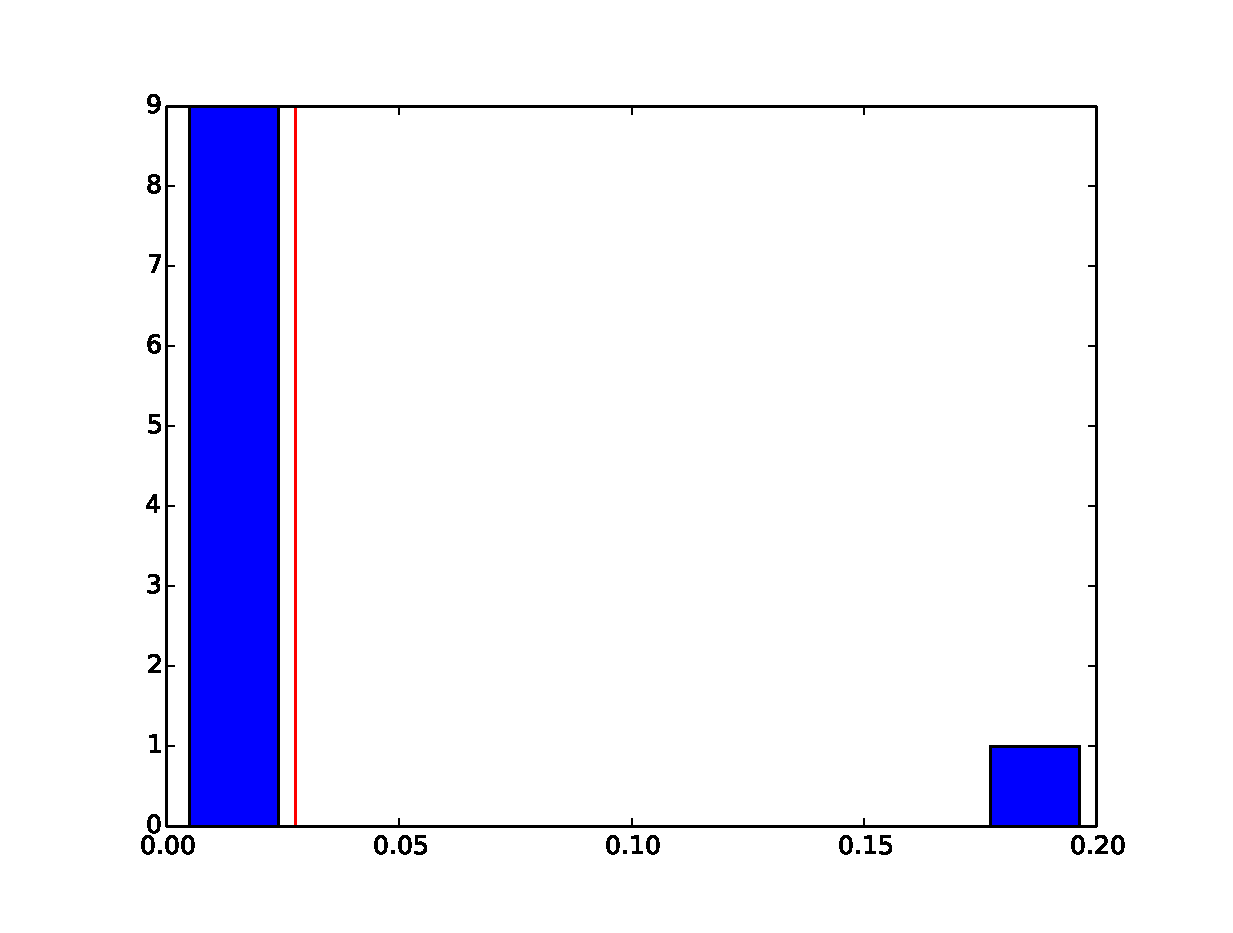
\includegraphics[width=\linewidth]{img/desktop_2_naive_3pt_dist_1.eps}
          \caption{Translation error histogram, mean in red} 
          \label{fig:desktop_2_naive_3pt_dist_1}
  \end{subfigure}
  \caption{Results using Naive \textit{Place Finder} and 3pt  \textit{Real Pose Finder}}
\end{figure}

In the case of the naive approach, in~\ref{fig:desktop_2_naive_3pt_dist_1}, the results are very good. Using this method the pose of the frames is recovered, in most cases, perfectly yelling a very low mean error. There is one frame which was not correctly relocalized, in that case not enough match were found between the pair of images. As seen in~\ref{fig:not_enough_matches} only two matches where found and , even correct, these are not enough to run the three-point algorithm. A large change in viewpoint can affect severely the descriptors performance been this the cause of the missing matches.\\

\begin{figure}[htpb]
  \centering
  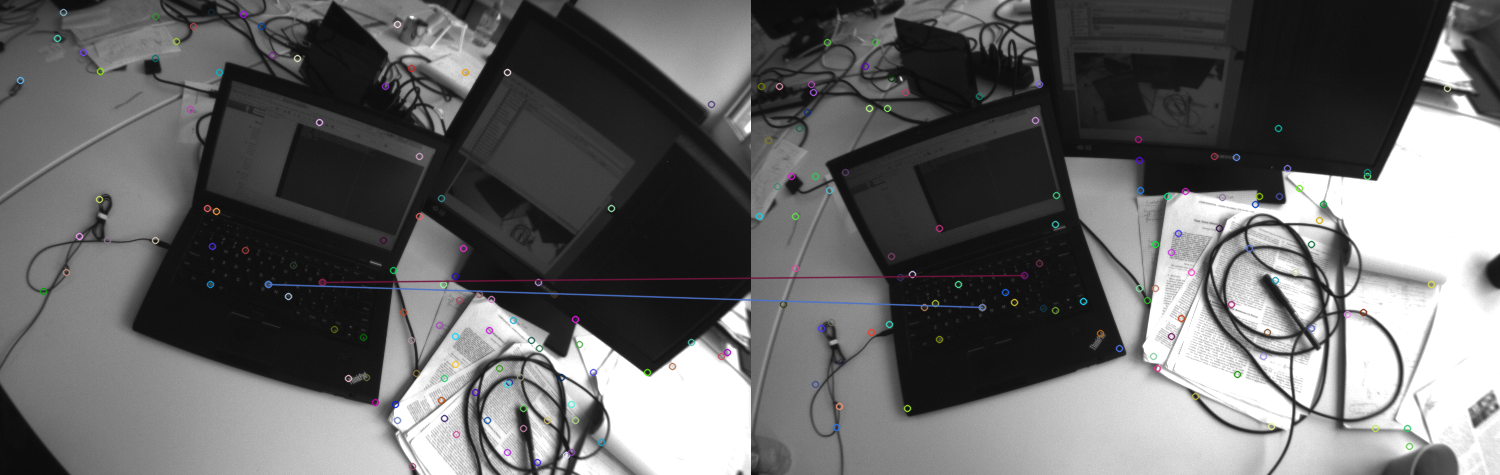
\includegraphics[width=11cm]{img/not_enough_matches.png}
  \caption{Found matches. Not enough to run the three-point algorithm}
  \label{fig:not_enough_matches}
\end{figure}

On the other case~\ref{fig:desktop_2_CC_3pt_dist_1}, using CC, the results are also good. Here, there is one of the frames whose pose is not correctly recovered. In this case, as seen in~\ref{fig:wrong_inlier}, there are enough matches but during RANSAC one match from three is taken in as valid leading to a wrong solution.\\

\begin{figure}[htpb]
  \begin{subfigure}[b]{6cm}
          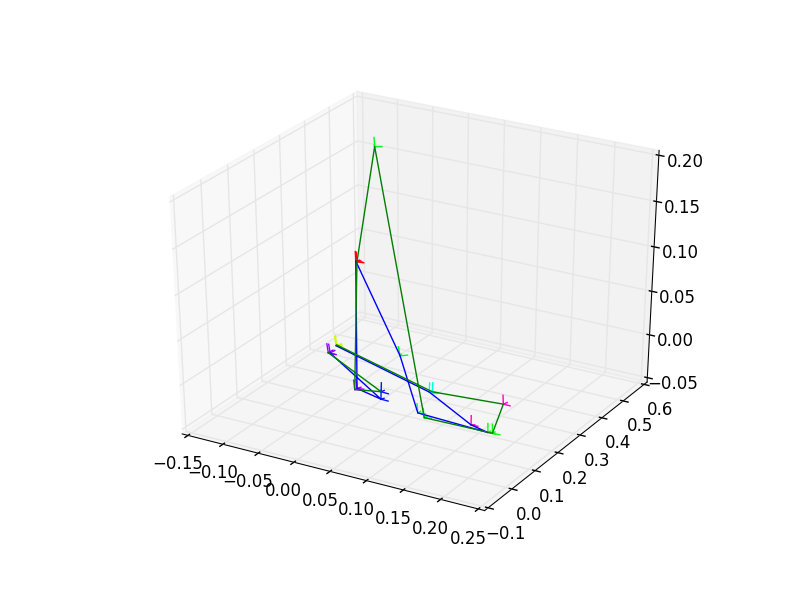
\includegraphics[width=\linewidth]{img/desktop_2_CC_3pt_path_1.png}
          \caption{In blue, testing ground truth. In green, found path}                
          \label{fig:desktop_2_CC_3pt_path_1}
  \end{subfigure}   
  \qquad
  \begin{subfigure}[b]{6cm}
          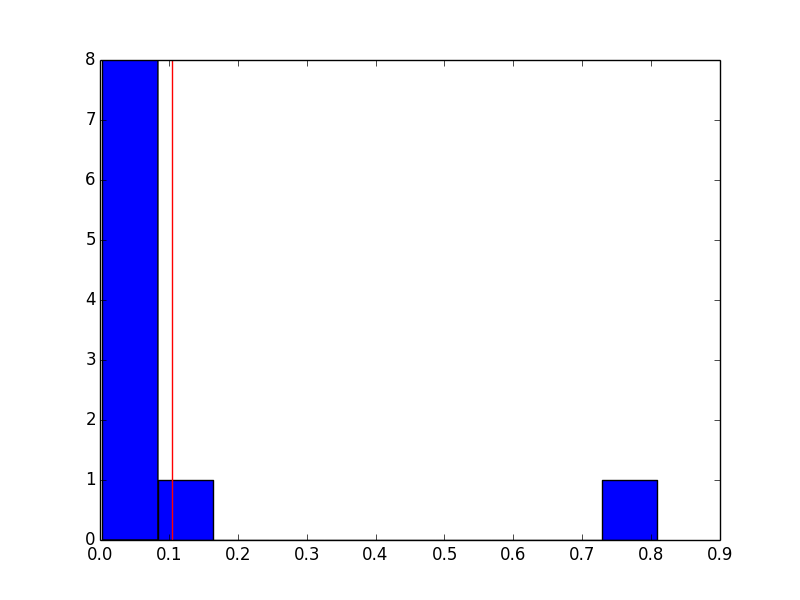
\includegraphics[width=\linewidth]{img/desktop_2_CC_3pt_dist_1.png}
          \caption{Translation error histogram, mean in red} 
          \label{fig:desktop_2_CC_3pt_dist_1}
  \end{subfigure}
  \caption{Results using CC \textit{Place Finder} and 3pt  \textit{Real Pose Finder}}
\end{figure}

\begin{figure}[htpb]
  \centering
  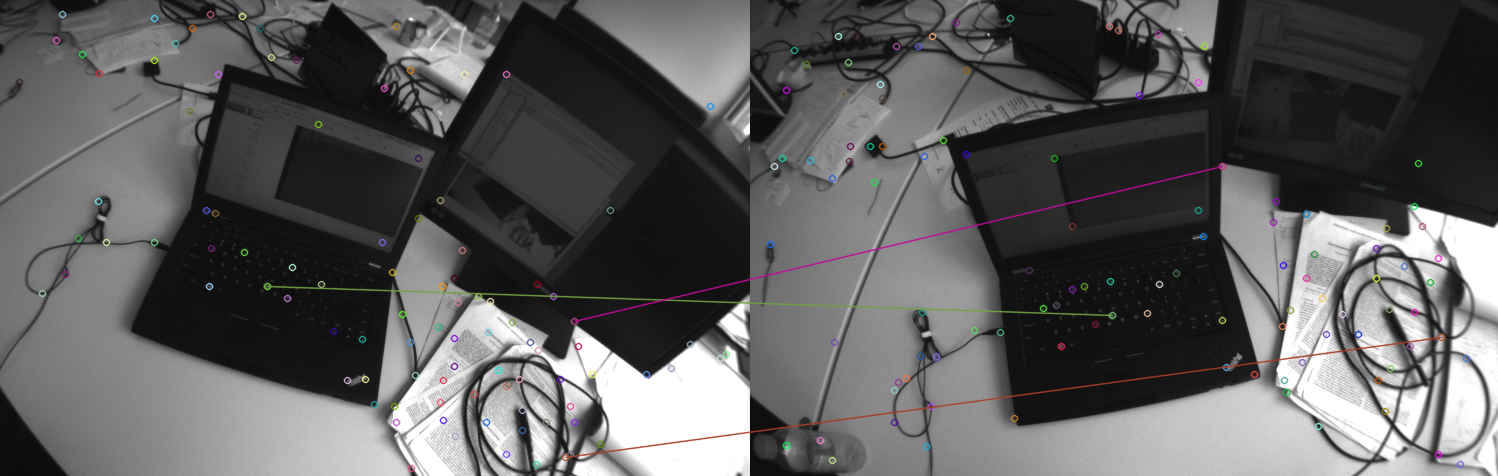
\includegraphics[width=11cm]{img/wrong_inlier.png}
  \caption{Example of accepted wrong match after RANSAC}
  \label{fig:wrong_inlier}
\end{figure}


\subsection{Ferns}
\label{sub:ferns_results}

Finally, as an alternative to the PTAM relocalization method, it was proposed to use machine learning techniques, more concretely \textit{ferns}~\cite{Ozuysal2010}. As seen in~\ref{fig:desktop_2_ferns_dist_1} in this simple example it performs well having a very low mean error.\\

When comparing the found path in~\ref{fig:desktop_2_ferns_path_1} with the found with the Multi relocalizer with three-point it seems that it is not as precise, but in this case all frames where well relocalized. The three-point \textit{Real Pose Finder} works very well locally yelling precise results when good matches are found, but it is very dependent on the results of the \textit{Place Finder}, on the other hand the \textit{ferns} relocalizer works globally. This makes it performs better in some cases but is a problem when scaling to larger environments.\\

In this example 237 classes are used (one per world point). It should be noticed that not all points need to be well classified, as long as more than 3 points are correctly identified then the posterior RANSAC will find and use the once that agree.\\


\begin{figure}[htpb]
  \begin{subfigure}[b]{6cm}
          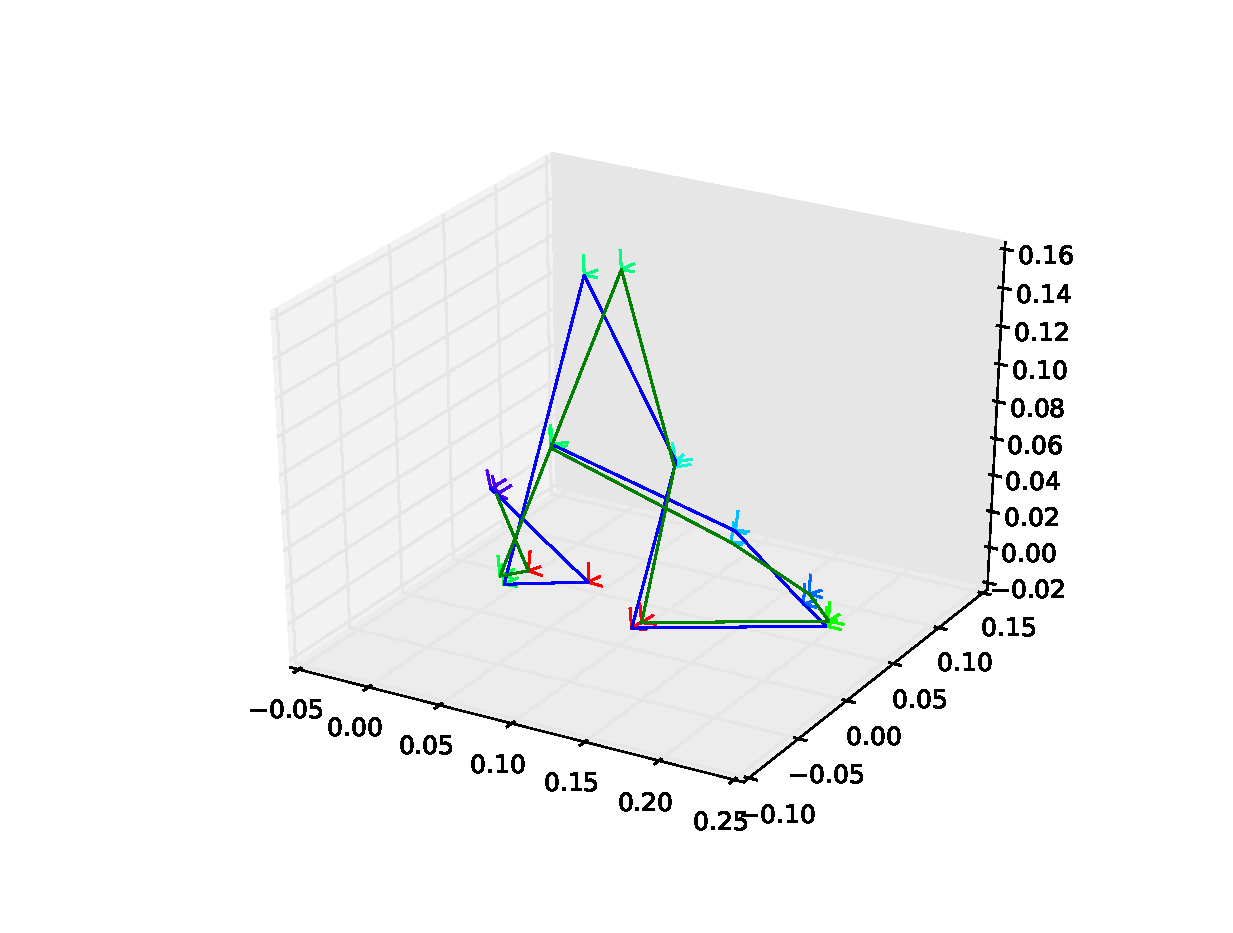
\includegraphics[width=\linewidth]{img/desktop_2_ferns_60_12_path_1.eps}
          \caption{In blue, testing ground truth. In green, found path}                
          \label{fig:desktop_2_ferns_path_1}
  \end{subfigure}   
  \qquad
  \begin{subfigure}[b]{6cm}
          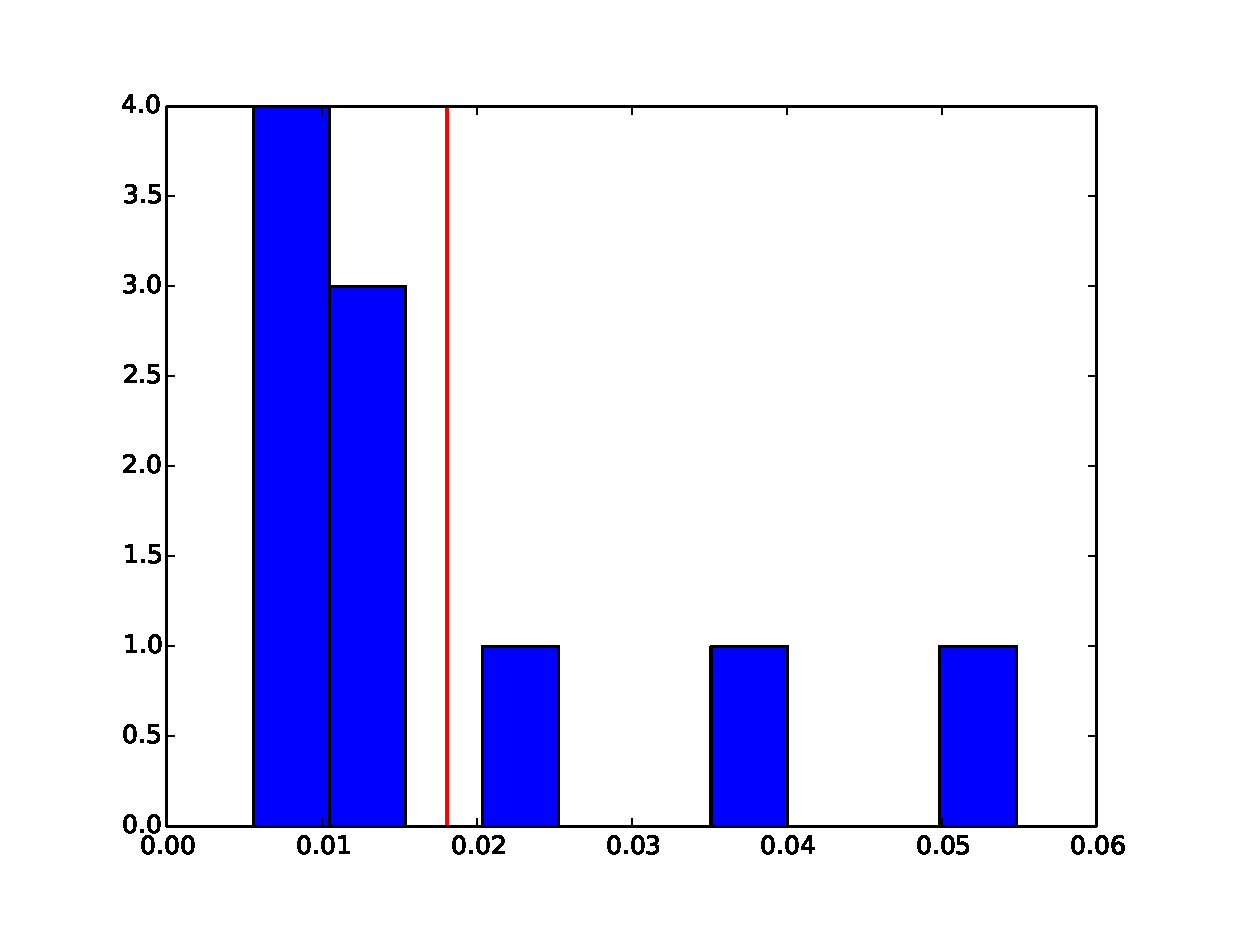
\includegraphics[width=\linewidth]{img/desktop_2_ferns_60_12_dist_1.eps}
          \caption{Translation error histogram, mean in red} 
          \label{fig:desktop_2_ferns_dist_1}
  \end{subfigure}
  \caption{Results using \textit{ferns} with 12 tests}
\end{figure}


\section{Large Dataset}
\label{sec:large_dataset}

As a second experiment a larger scenario has been closed. It is also desktop, but in this case, covering an area of 7x3 meters. The taken path to acquire training and testing data covering the mentioned area can be seen in~\ref{fig:large_desktop_train_test} while in Figure~\ref{fig:large_desktop_example_image} there is an example of the dataset images. The dataset contains 84 frames for training and 69 for testing.\\

\begin{figure}[htpb]
  \begin{subfigure}[b]{6cm}
          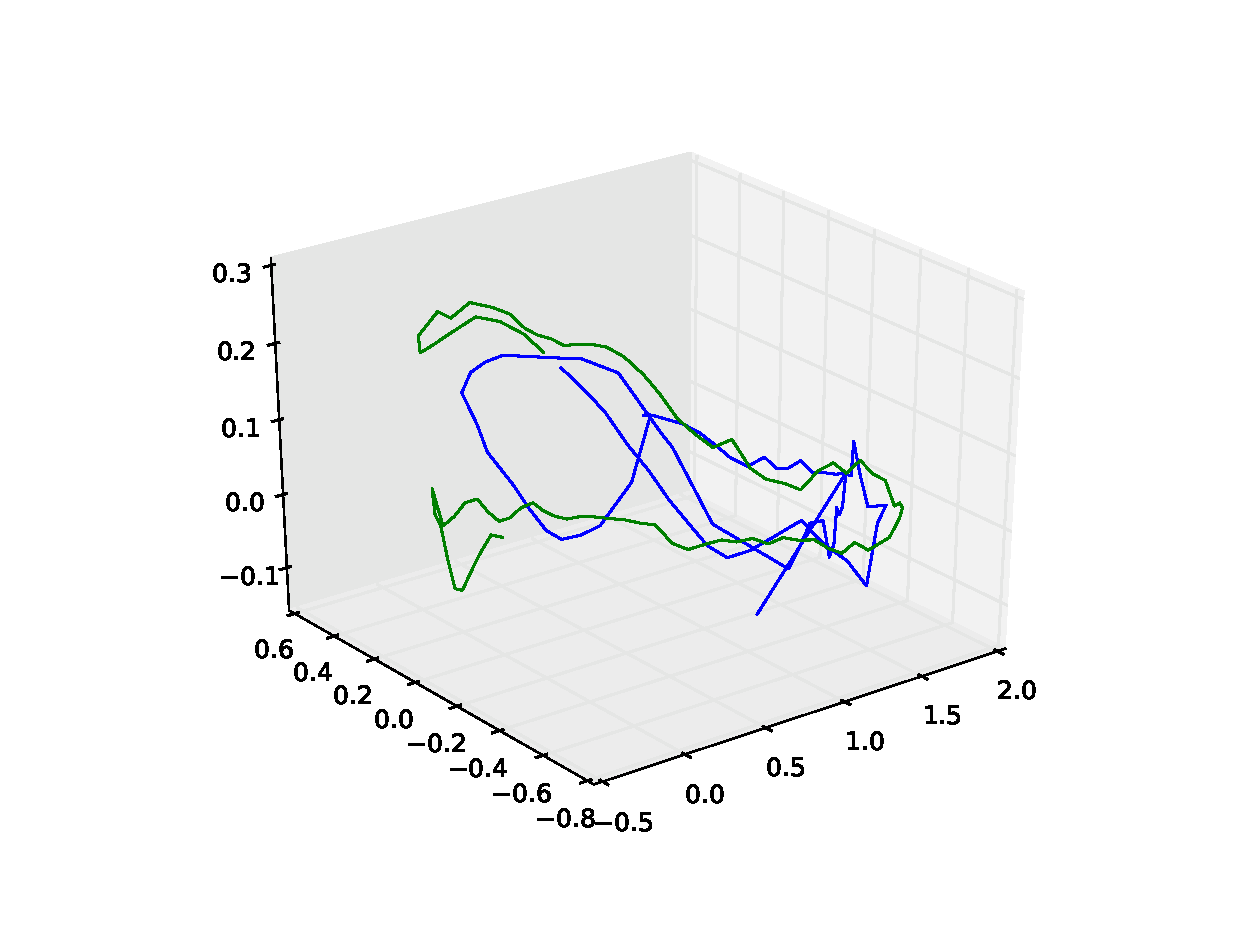
\includegraphics[width=\linewidth]{img/large_desktop/test_train_path.eps}
          \caption{In green, the path used for training. In blue, the path used for testing}                
          \label{fig:large_desktop_train_test}
  \end{subfigure}   
  \qquad
  \begin{subfigure}[b]{5cm}
         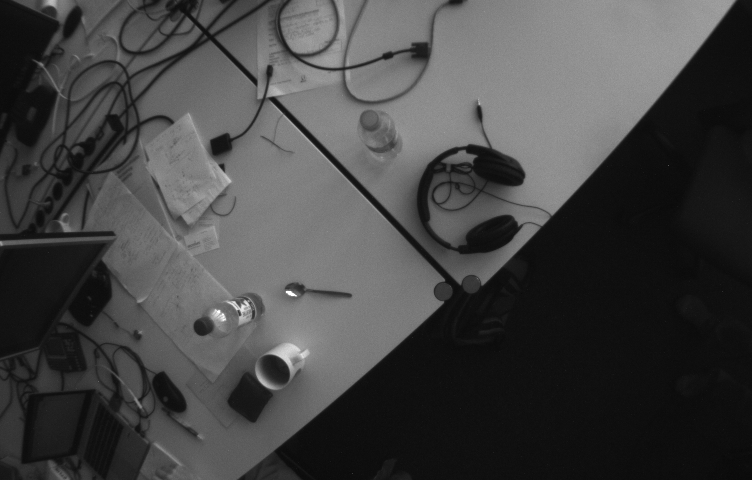
\includegraphics[width=\linewidth]{img/large_desktop/image00778.png}
         \caption{Example of an image from the dataset}                
         \label{fig:large_desktop_example_image}
  \end{subfigure}
  \caption{}
\end{figure}

\subsection{Multi Relocalizer}
\label{sub:multi_relocalizer_large}

\subsubsection{Naive and CC \textit{Place finder}}
\label{ssub:naive_and_cc_place_finder_large}

First of all, again, it performance of the \textit{Place Finder} is analysed to see then how posterior processes can improve it. In this case the Naive method gives a good baseline as was expected. On the other side, CC, have some good associations that seem to agree to Naive's with errors between 0.05 and 0.25, but it also has some wrong associations which probably cannot be corrected for example the one seen in~\ref{fig:large_CC_wrong_asociation}.\\

\begin{figure}[htpb]
  \begin{subfigure}[b]{6cm}
          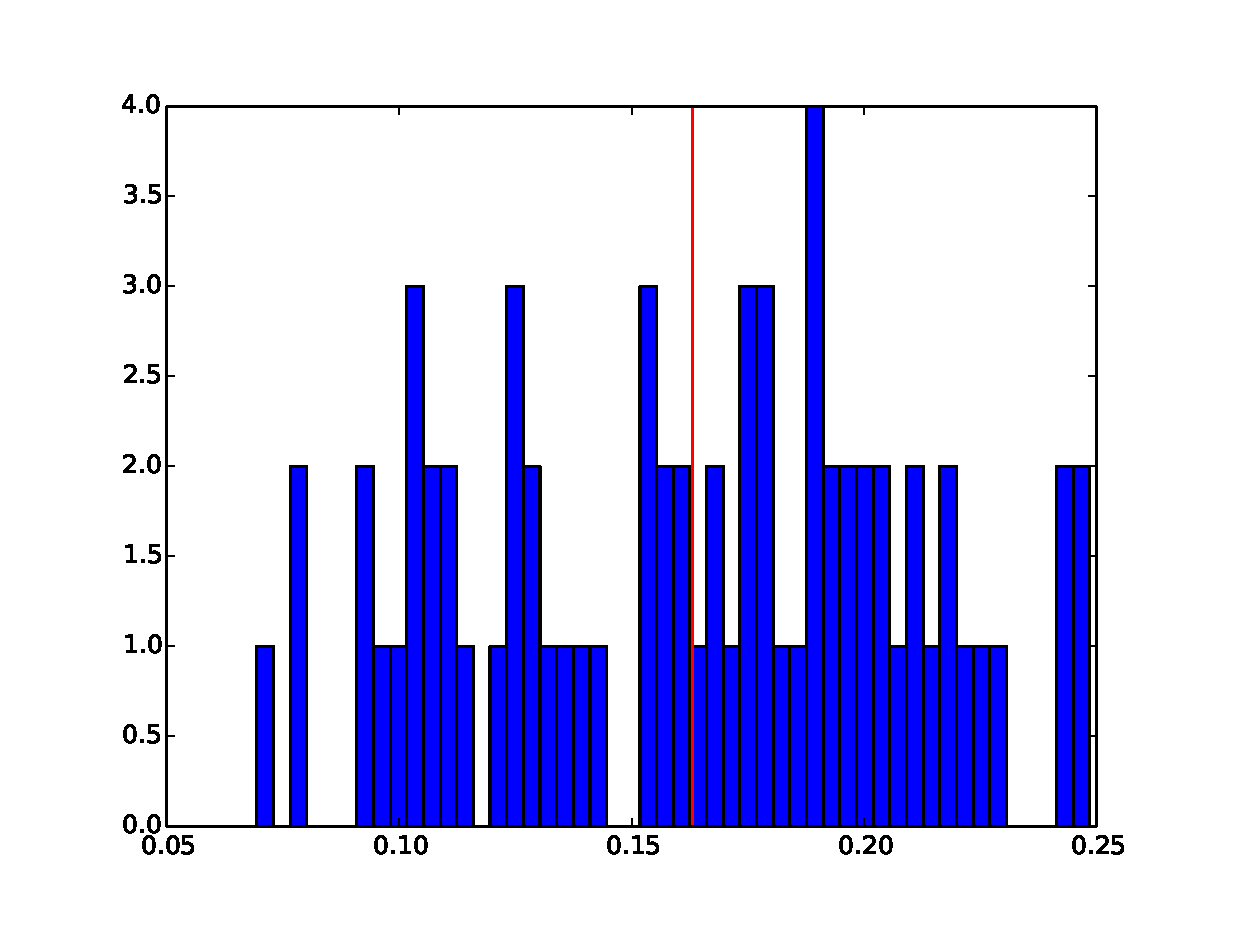
\includegraphics[width=\linewidth]{img/large_desktop/naive_empty_dist.eps}
          \caption{Naive \textit{Place Finder} translation error histogram}                
          \label{fig:large_naive_empty_dist}
  \end{subfigure}   
  \qquad
  \begin{subfigure}[b]{6cm}
         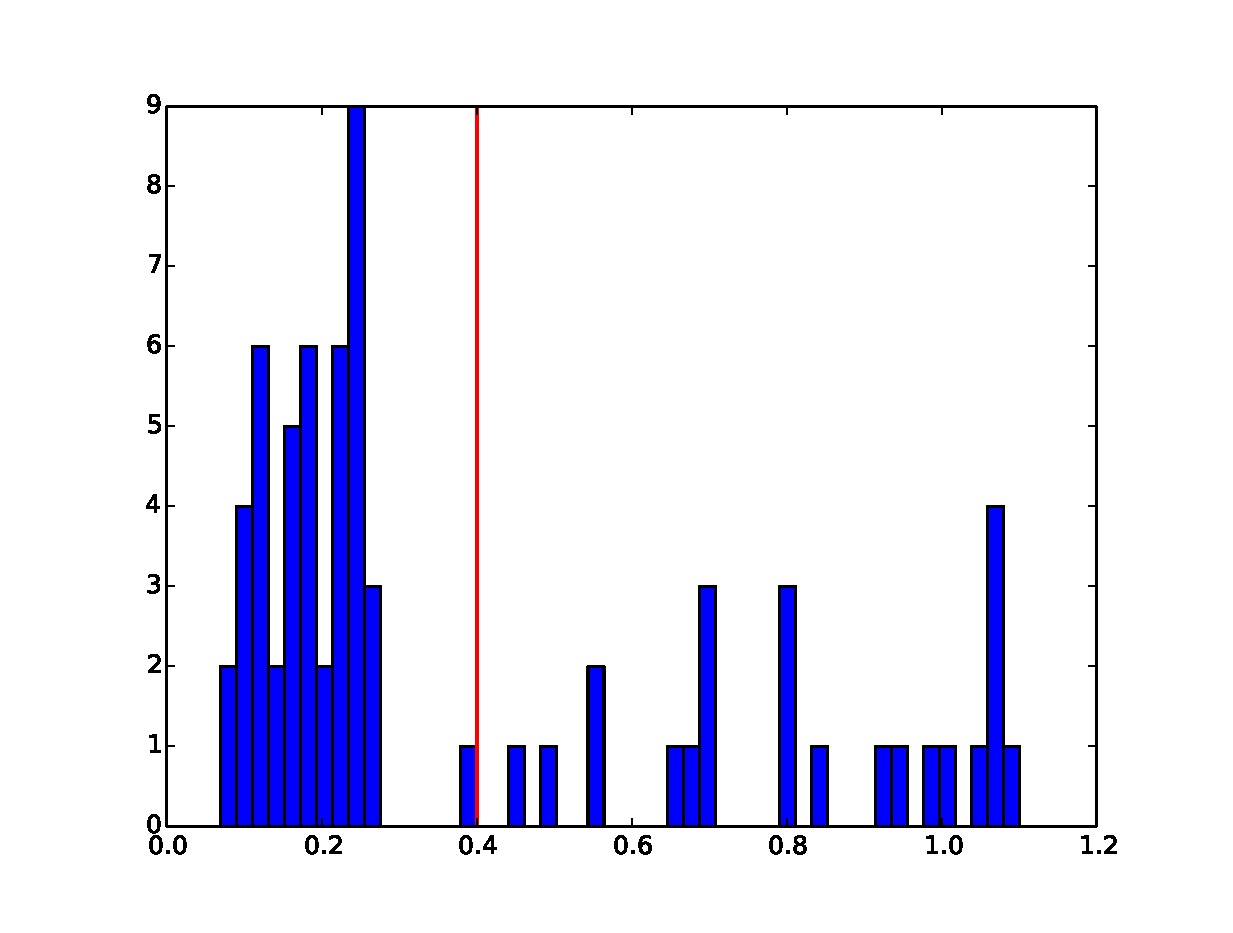
\includegraphics[width=\linewidth]{img/large_desktop/CC_empty_dist.eps}
         \caption{CC \textit{Place Finder} translation error histogram}                
         \label{fig:large_CC_empty_dist}
  \end{subfigure}
  \caption{}
  \label{fig:large_place_finder_dist}
\end{figure}

\begin{figure}[htpb]
  \centering
  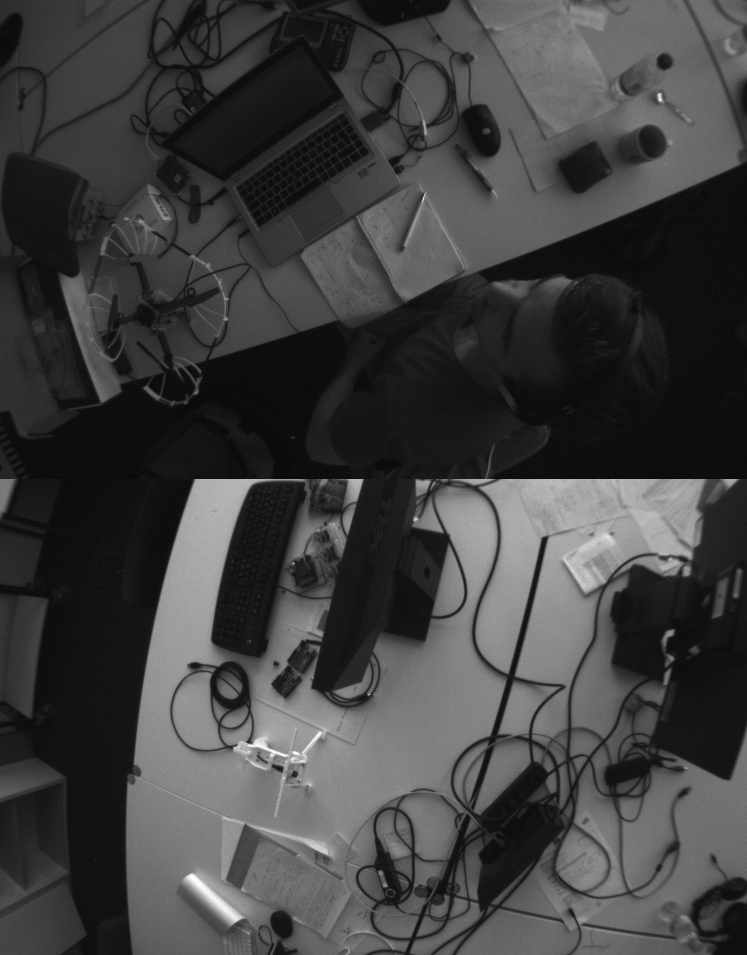
\includegraphics[width=8cm]{img/large_desktop/CC_wrong_asociation.png}
  \caption{CC wrong association}
  \label{fig:large_CC_wrong_asociation}
\end{figure}


\subsubsection{Extended Second-order Minimization \textit{Real Pose Finder}}
\label{ssub:extended_second_orther_minimization_real_pose_finder}

In this case the produced path plot have also been avoided because they did not contribute with understandable visual information. Looking at the error distributions and comparing them to the performance from~\ref{fig:large_place_finder_dist} it seems that together with the Naive \textit{Place Finder} it worsen the results while with CC the results are similar, maybe slightly better. In general this method does not seem to apply well on this dataset. \\

\begin{figure}[htpb]
  \begin{subfigure}[b]{6cm}
          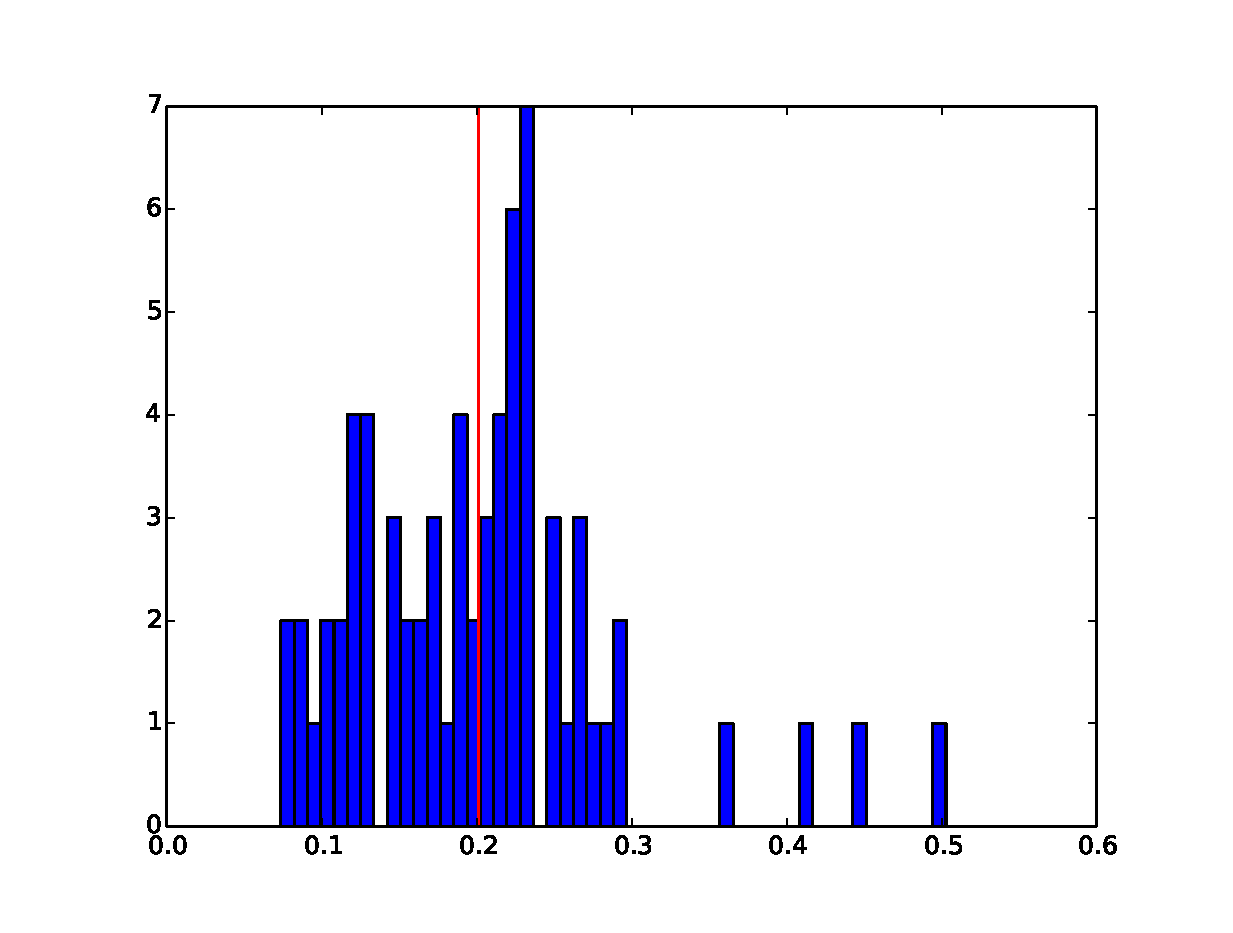
\includegraphics[width=\linewidth]{img/large_desktop/naive_esm_dist.eps}
          \caption{Translation error histogram using Naive \textit{Place Finder} and ESM \textit{Real Pose Finder}}
          \label{fig:desktop_2_CC_3pt_path_1}
  \end{subfigure}   
  \qquad
  \begin{subfigure}[b]{6cm}
          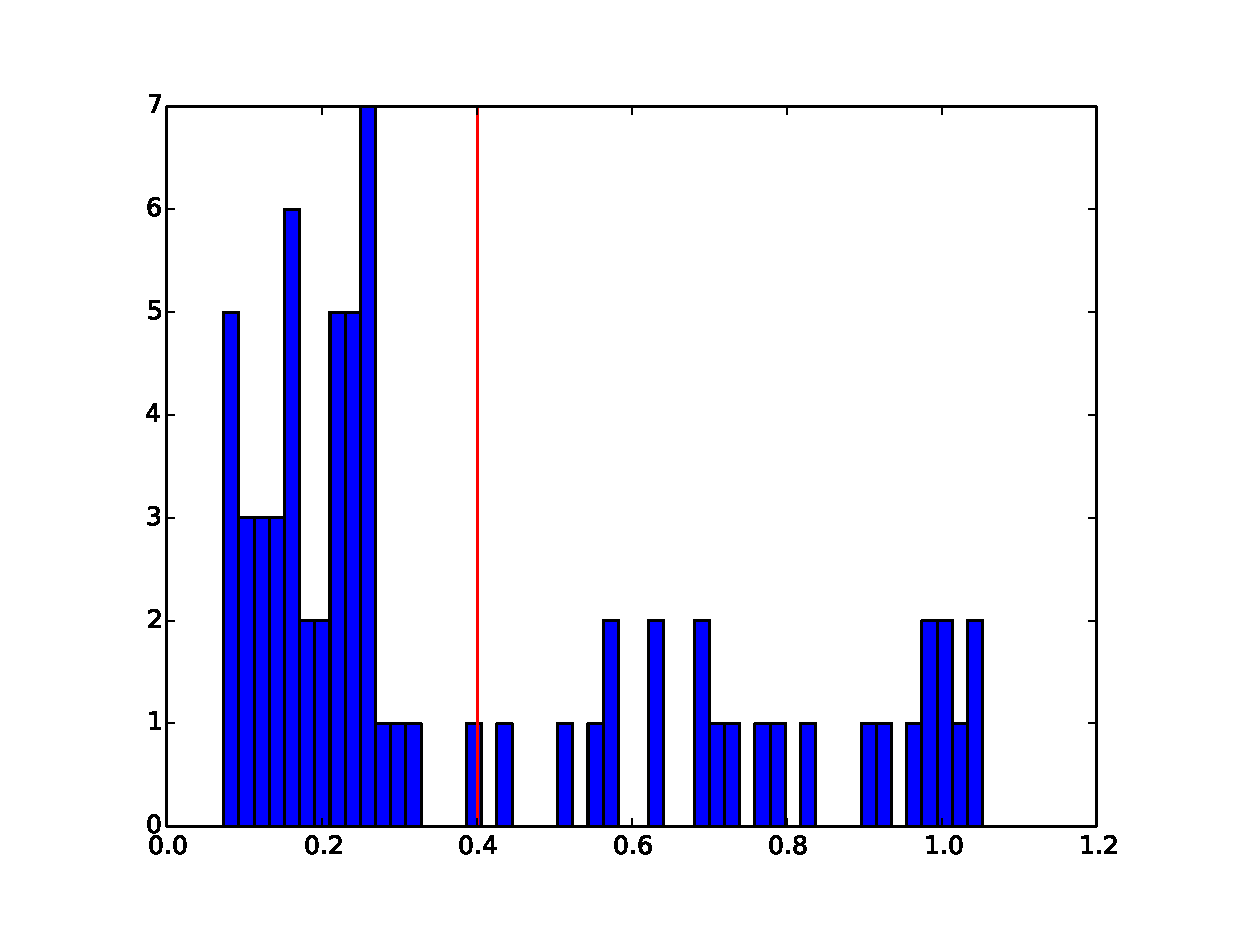
\includegraphics[width=\linewidth]{img/large_desktop/CC_esm_dist.eps}
          \caption{Translation error histogram using CC \textit{Place Finder} and ESM \textit{Real Pose Finder}}
          \label{fig:desktop_2_CC_3pt_dist_1}
  \end{subfigure}
  \caption{}
\end{figure}


\subsubsection{Three-point \textit{Real Pose Finder}}
\label{ssub:large_three_point_real_pose_finder}

On the other side, the Three-point \textit{Real Pose Finder} seems to work very well with this dataset. Using the Naive \textit{Place Finder} it is able to correctly find the pose of every frame. Using CC the results are also acceptable good correctly retrieving the pose of 42 of the 69 frames. As said before, and it can be seen again in this case, this method is very dependent on the results of the \textit{Place Finder} and on this dataset CC was not very effective.\\

\begin{figure}[htpb]
  \begin{subfigure}[b]{6cm}
          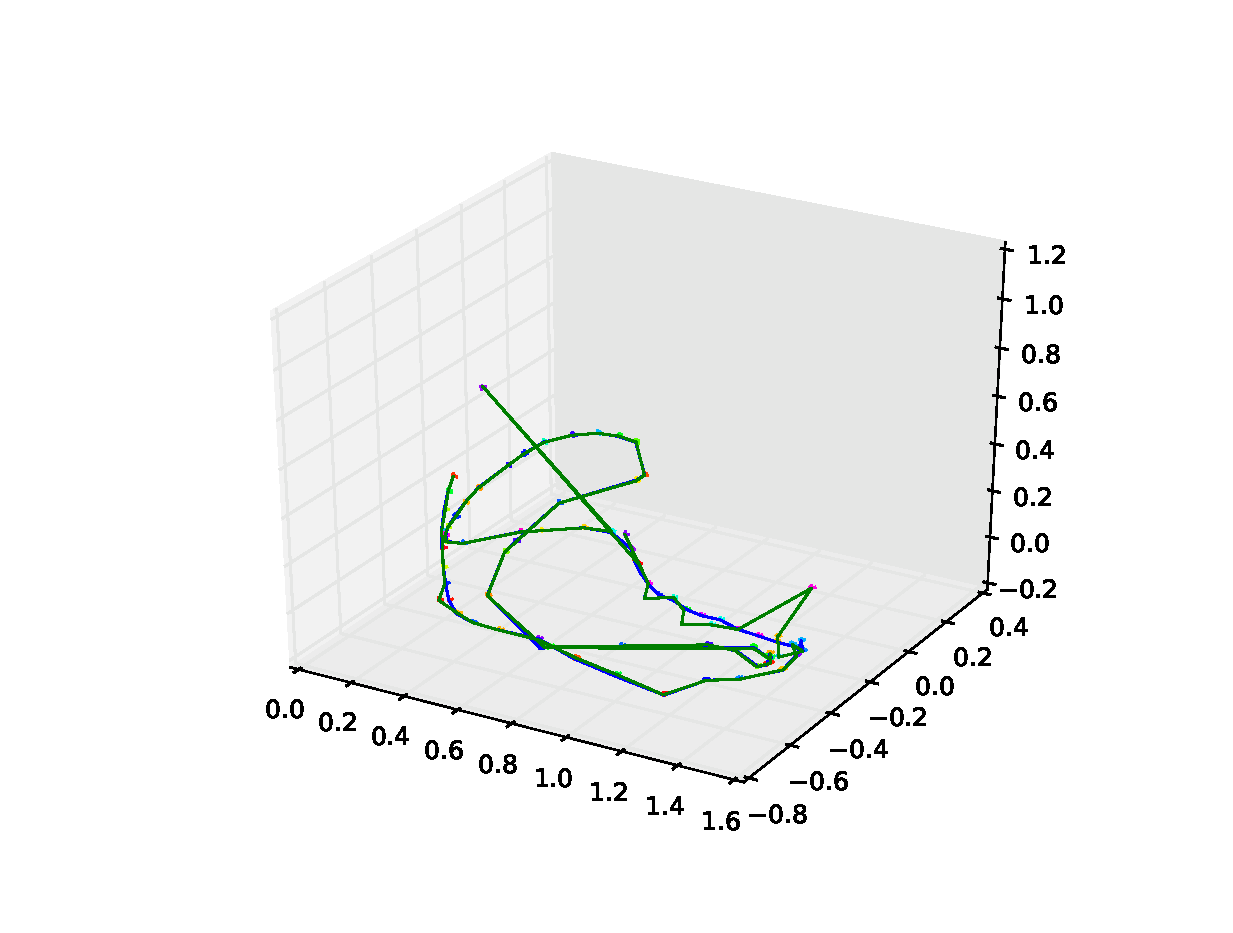
\includegraphics[width=\linewidth]{img/large_desktop/naive_3pt_path.eps}
          \caption{In blue, testing ground truth. In green, found path}                
          \label{fig:desktop_2_ferns_path_1}
  \end{subfigure}   
  \qquad
  \begin{subfigure}[b]{6cm}
          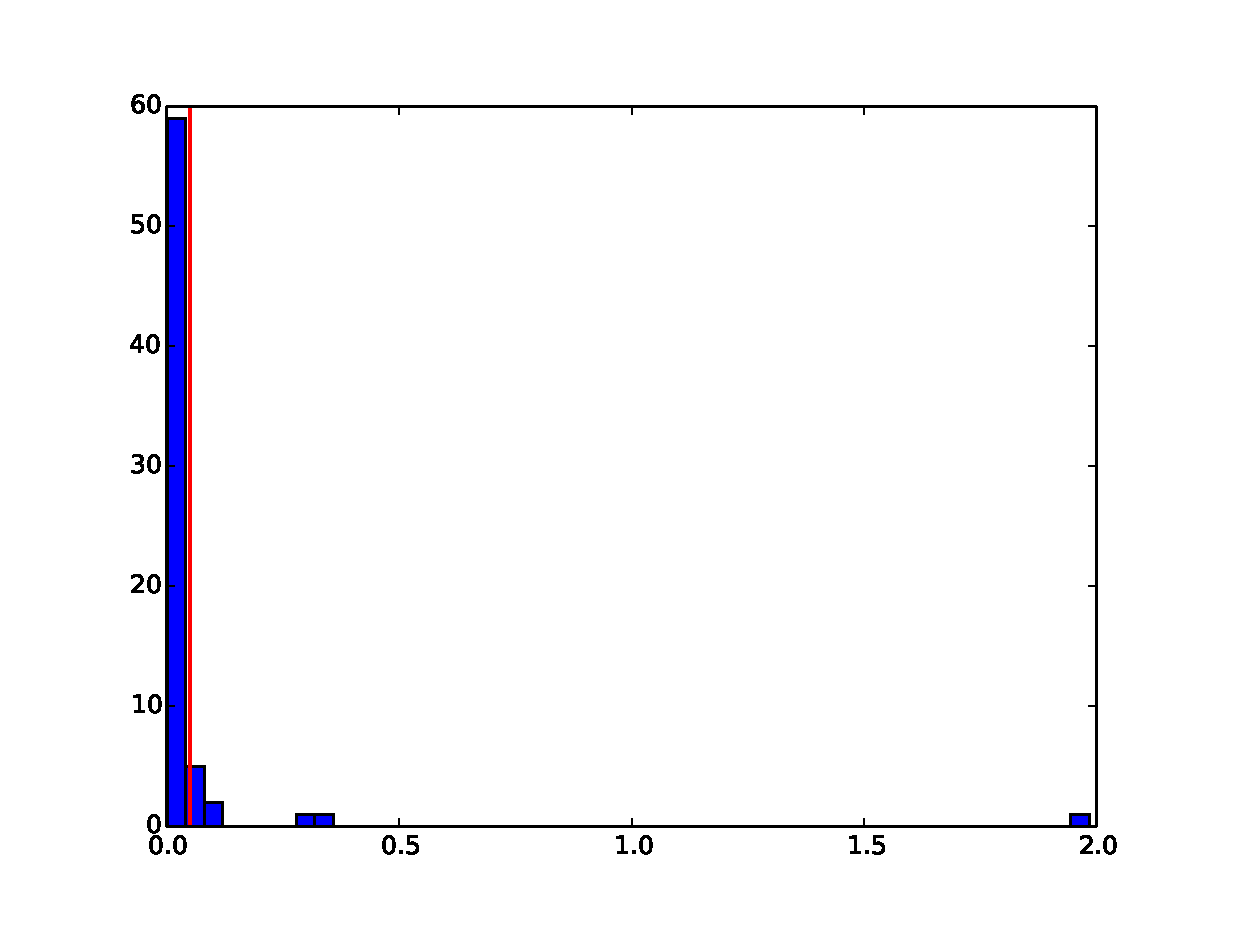
\includegraphics[width=\linewidth]{img/large_desktop/naive_3pt_dist.eps}
          \caption{Translation error histogram, mean in red} 
          \label{fig:desktop_2_ferns_dist_1}
  \end{subfigure}
  \caption{Results using Naive and 3pt on a larger dataset}
\end{figure}

\begin{figure}[htpb]
  \begin{subfigure}[b]{6cm}
          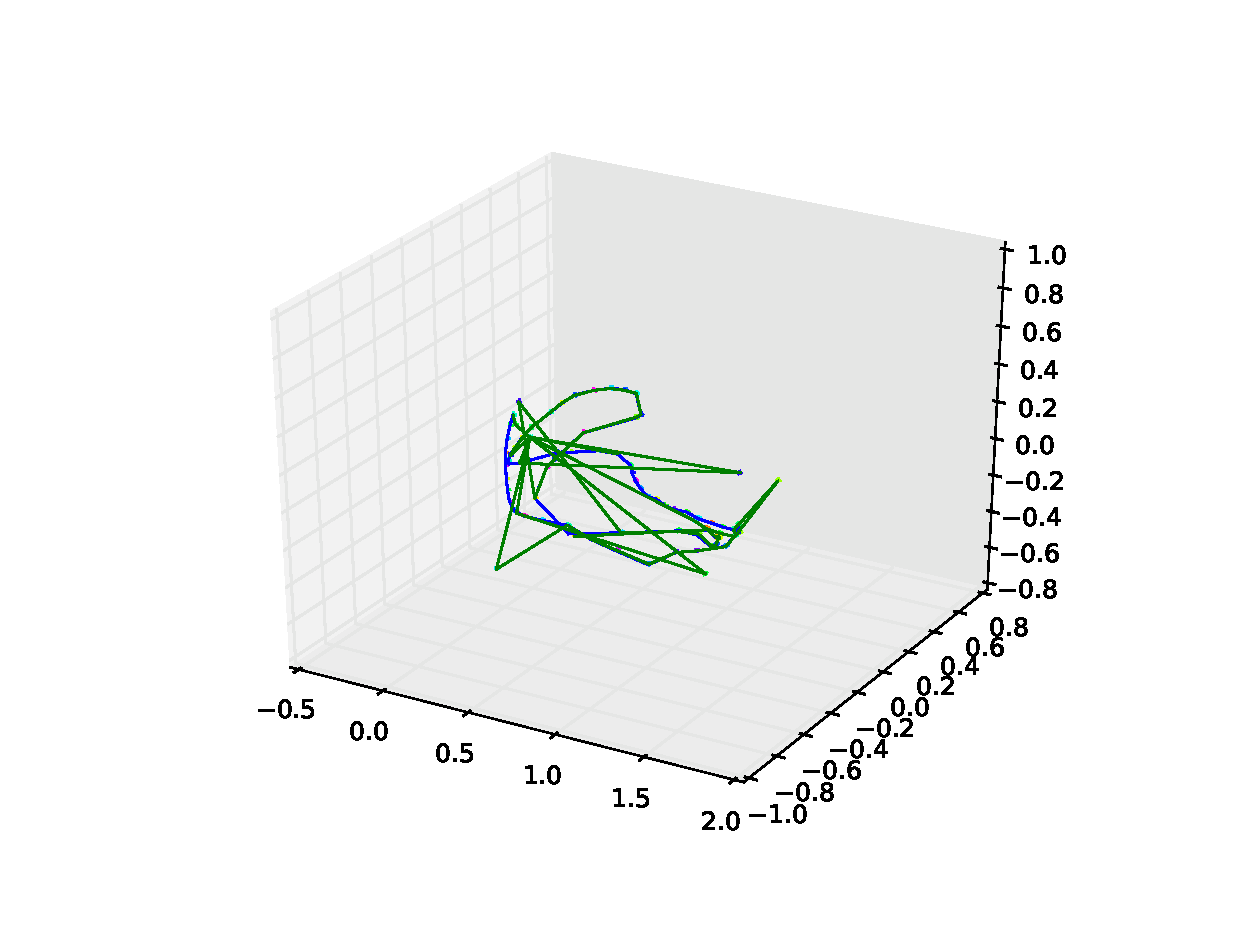
\includegraphics[width=\linewidth]{img/large_desktop/CC_3pt_path.eps}
          \caption{In blue, testing ground truth. In green, found path}                
          \label{fig:desktop_2_ferns_path_1}
  \end{subfigure}   
  \qquad
  \begin{subfigure}[b]{6cm}
          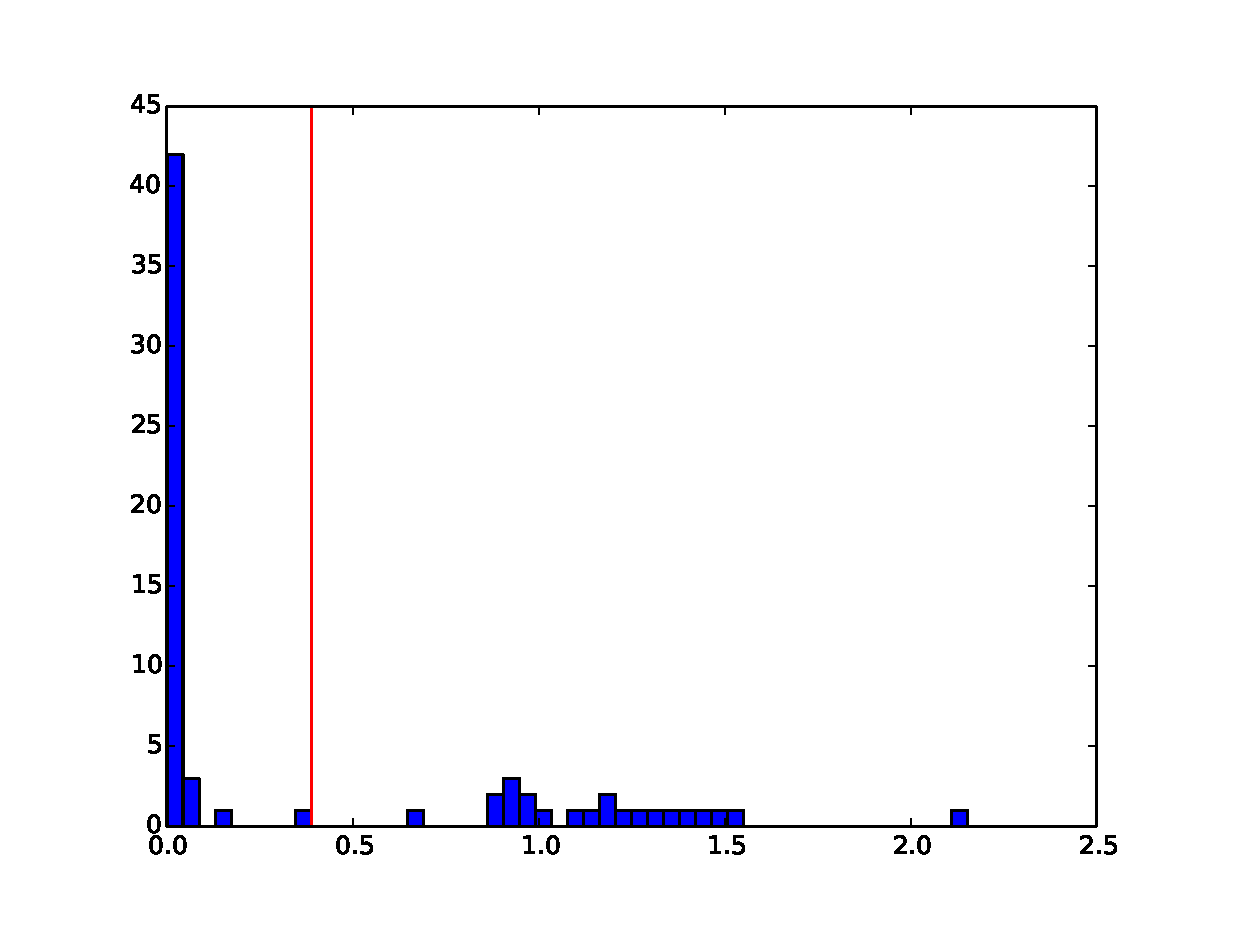
\includegraphics[width=\linewidth]{img/large_desktop/CC_3pt_dist.eps}
          \caption{Translation error histogram, mean in red} 
          \label{fig:desktop_2_ferns_dist_1}
  \end{subfigure}
  \caption{Results using CC and 3pt on a larger dataset}
\end{figure}


\subsection{Ferns}
\label{sub:large_ferns}

In~\cite{Ozuysal2010} it is said that \textit{fenrs} can be used to distinguish up to around 200 different classes. We applied the method to this dataset where there are 1730 classes. In~\ref{fig:large_desktop_ferns_dist} shows that almost 50 of the 69 frames where correctly relocalized. That is, more than using Multi Relocalizer with the three-point \textit{Real Pose Finder}. The classifier was trained with 100 \textit{ferns} of 12 tests each.\\

It is interesting to see that both methods, three-point with CC and this one, can correctly relocalize the same number of frames. Probably there is one part of the dataset that is more ambiguous and difficult to recognize and both algorithms struggle with it (basically CC because it have been seen that three-point can correctly relocalize with the Naive \textit{Place Finder} which uses ground truth data).

\begin{figure}[htpb]
  \begin{subfigure}[b]{6cm}
          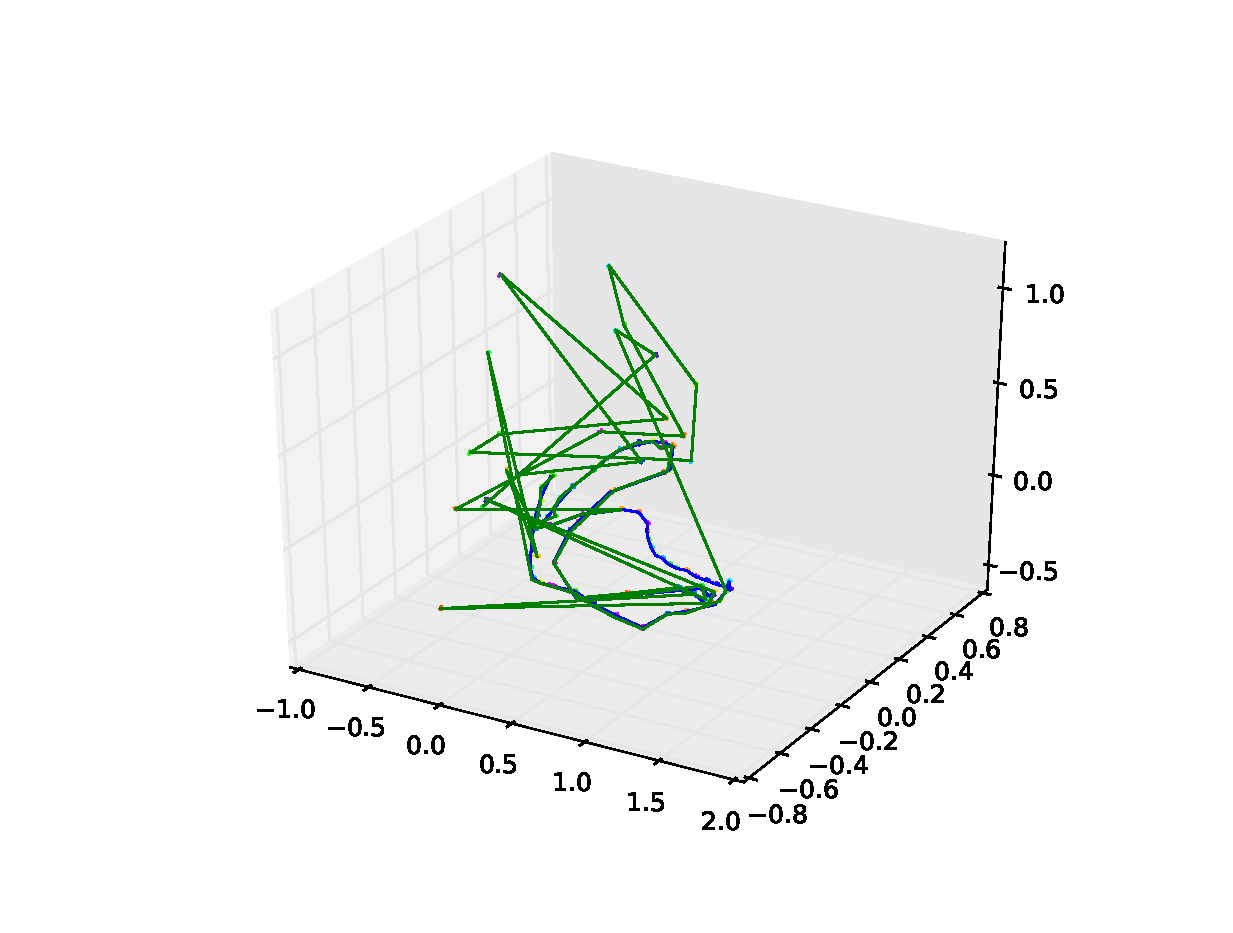
\includegraphics[width=\linewidth]{img/large_desktop/ferns_100_path.eps}
          \caption{In blue, testing ground truth. In green, found path}                
          \label{fig:large_desktop_ferns_path}
  \end{subfigure}   
  \qquad
  \begin{subfigure}[b]{6cm}
          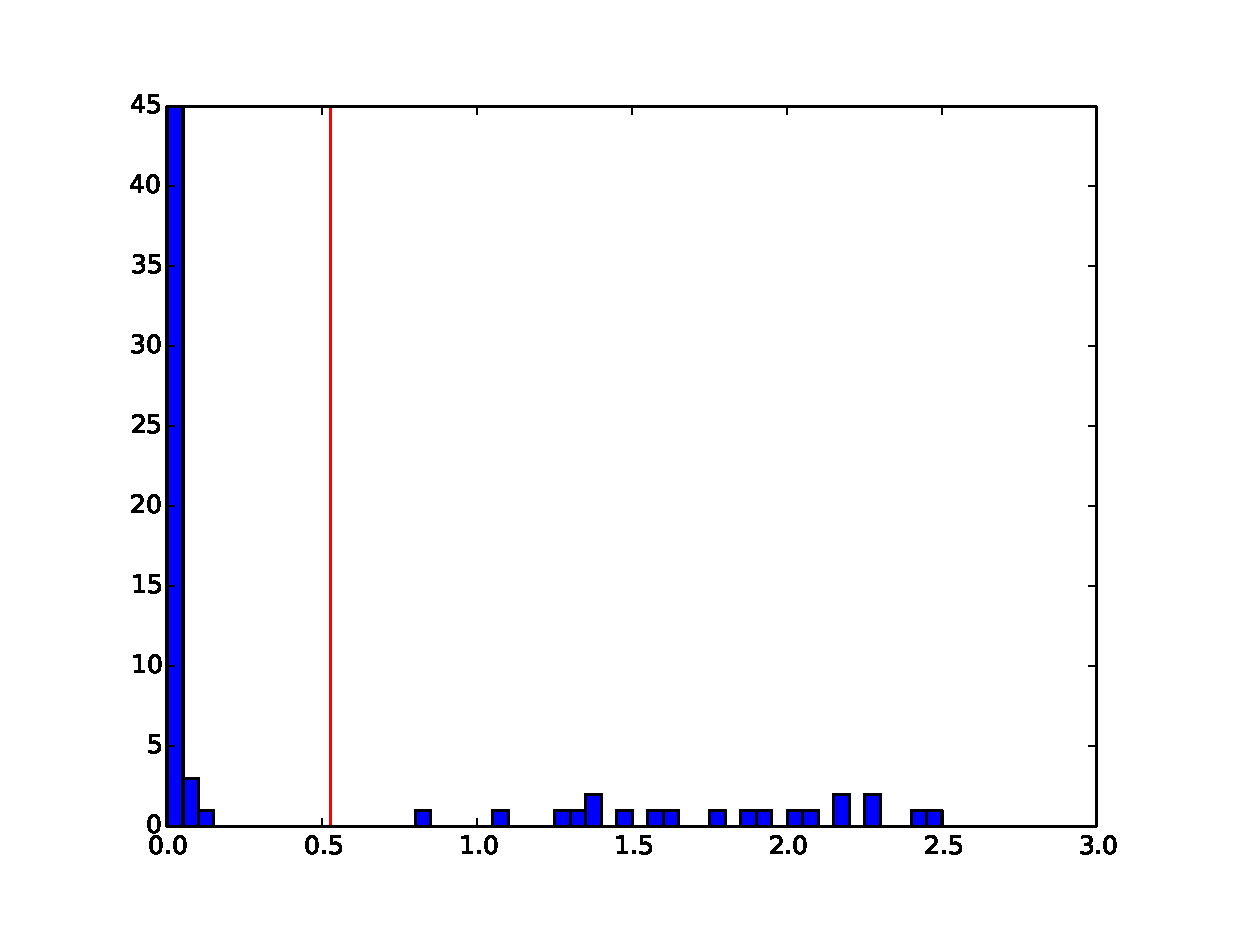
\includegraphics[width=\linewidth]{img/large_desktop/ferns_100_dist.eps}
          \caption{Translation error histogram, mean in red} 
          \label{fig:large_desktop_ferns_dist}
  \end{subfigure}
  \caption{Results using \textit{ferns} with 12 tests}
\end{figure}


